\section{Results}

\begin{figure}[tph]
  \centering
  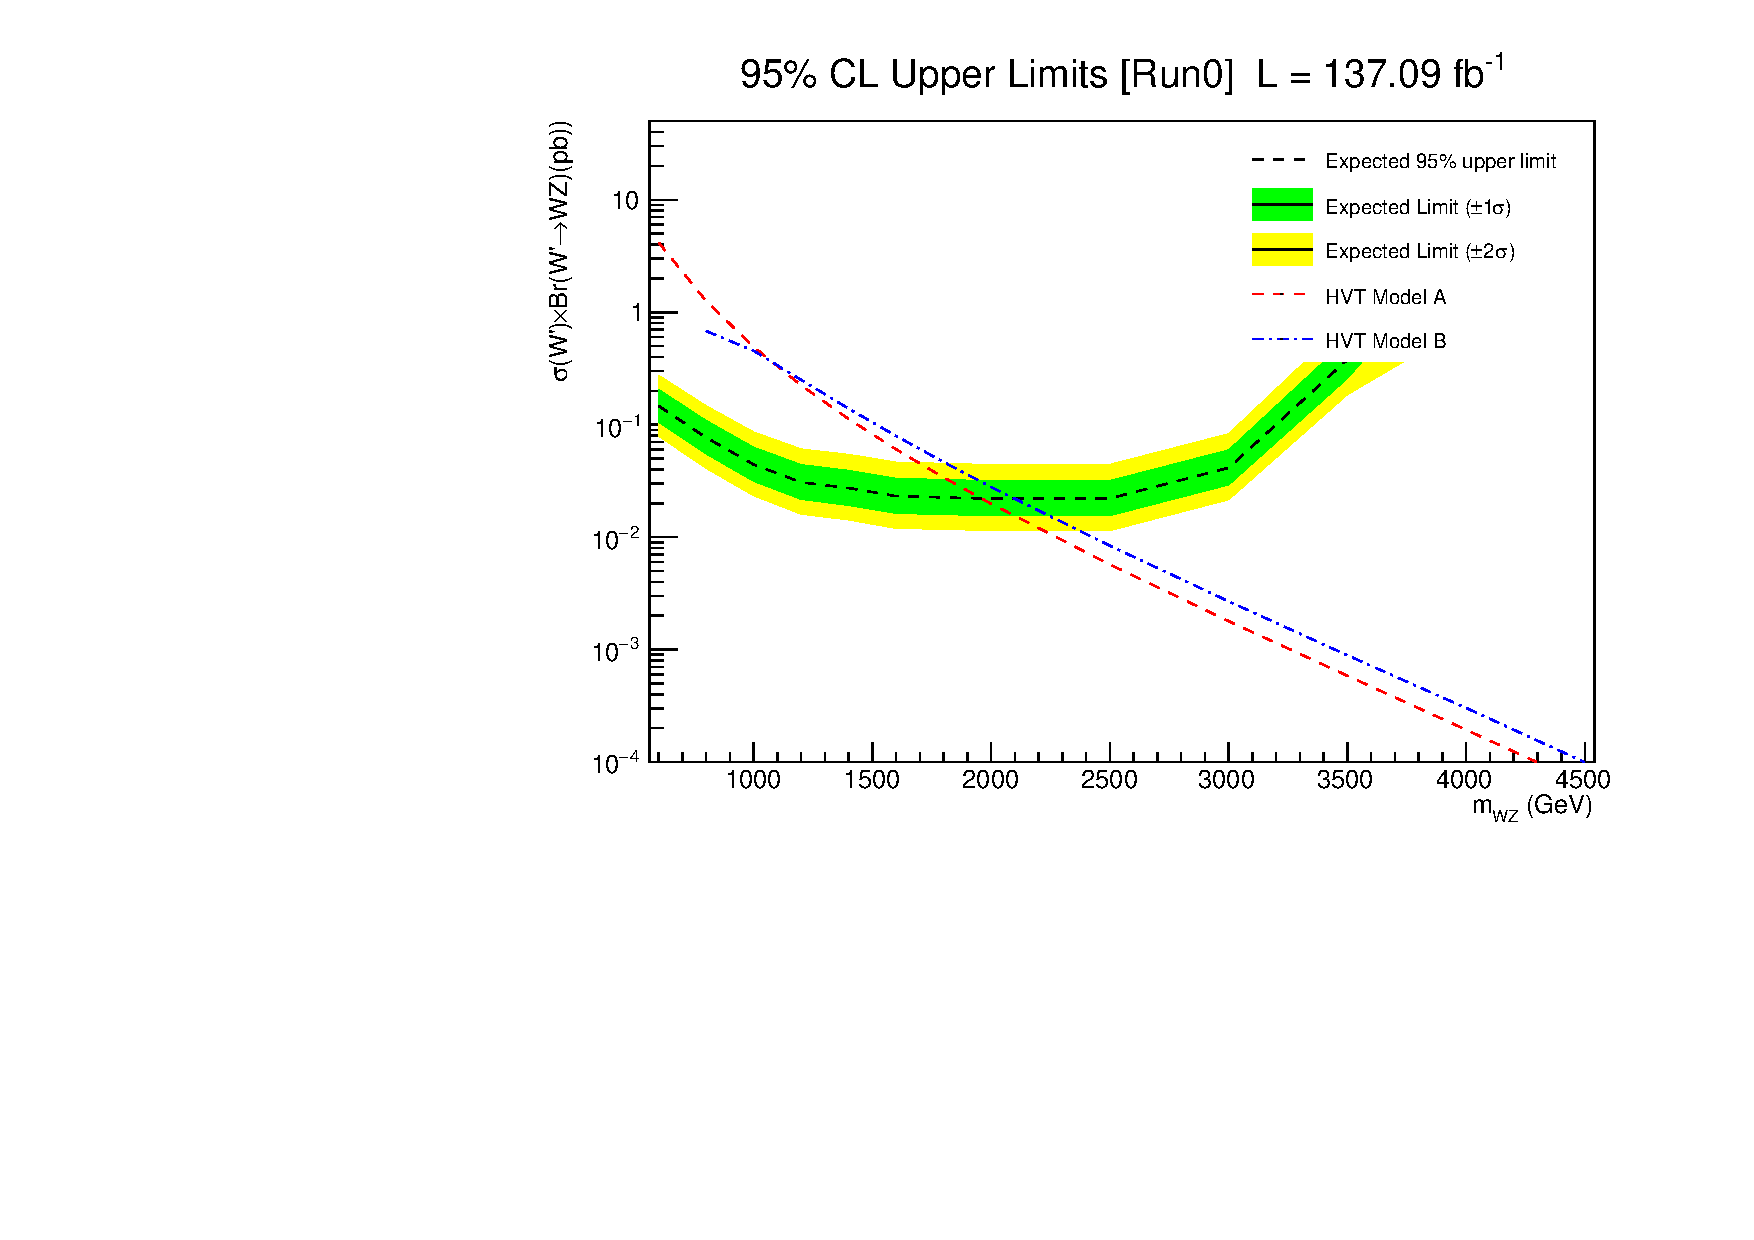
\includegraphics[width=0.6\textwidth]{fig/Run2/Run2_ExclusionLimits.pdf}
  \caption{95\% Confidence Level Upper Limits}
  \label{fig:BrazilianPlot}
\end{figure}

The \verb|RooStats| package is used to determine the 95\% confidence-level limit
on the signal contribution in the data. The \verb|AsymptoticLimits| method is
used with the CMS \verb|combine| tool to compute 95\% C.L upper-limits on the
production cross section times the branching ratio with one and two standard
deviation bands given by the frequentist calculation as recommended by the
Higgs Group.

Systematic uncertainties are considered nuisance parameters.

The expected upper limit on the resonance cross section times and its relative
68\% and 95\% uncertainty bands, are shown as a function of the resonant mass
in figure \ref{fig:BrazilianPlot}


